\documentclass[11pt,a4paper]{article}
\usepackage[left=2.5cm,right=2cm, bottom=2cm]{geometry}
\usepackage[utf8]{inputenc}
\usepackage{amsmath}
\usepackage{amsfonts}
\usepackage{amssymb}
\usepackage{amsfonts}
\usepackage{amsmath}
\usepackage{graphicx}
\usepackage{subfigure}
\usepackage{color}
\usepackage{abstract}
\usepackage{float}
\usepackage[toc,page]{appendix}
\usepackage{hyperref}
\usepackage{fancyhdr}
\usepackage{algorithm} 
\usepackage{algpseudocode} 
\usepackage{listings}
\usepackage{xcolor} % for setting colors
% set the default code style
\lstset{
	frame=tb, % draw a frame at the top and bottom of the code block
	tabsize=4, % tab space width
	showstringspaces=false, % don't mark spaces in strings
	numbers=left, % display line numbers on the left
	commentstyle=\color{green}, % comment color
	keywordstyle=\color{blue}, % keyword color
	stringstyle=\color{red} % string color
}

\pagestyle{fancy}
\fancyhf{}
\rhead{\today}
\lhead{\bfseries Alexander Leitner 01525882}
\rfoot{}



\begin{document}
%\begin{center}
%	\fontsize{24pt}{10pt}\selectfont
%	\textsc{\textbf{Experiment Design for Data Science  Exercise 1}}
%\end{center}
\section{Explore the data}
\subsection{Data explenarsion}
This dataset deals with the rating (1-5) of 1682 different films and classifier this films in several groups like (Children, Adventure,...). \\\\The first file (u.user) contain information from the film tester like their ages, sex or occupation. The data in this file are nominal(sex, occupation) and the other columns are numeric values.\\\\ For the nominal columns there could be ethnical problems. A solution for the age column could be that they can divide it into 4 parts to secure the information. For the sex column it is possible to decode it for example $"F" \rightarrow 1$ and $"M" \rightarrow 0$. So the reader could not know the gender and for the algorithm it does not change anything. For the third column it is also possible to divide this into other sections like "official", "private sector".\\\\
The second file u.data contained only numerical values. The rating column is divided into \\(1-5) where 1 is the best and 5 is the worst.\\
The lastimportant file is (u.item). It has binary types for the classification the film, a column with only $nan$ values, nominal values (film names, Url sources) and dates.\\
The column with the $nan$ values could not predict because there is no way to do this only to look on the internet and add this information. 

\begin{minipage}[t]{0.33\textwidth}
	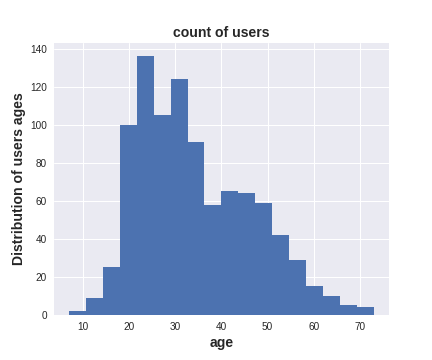
\includegraphics[width=\textwidth]{Bilder/age_dist.png}
\end{minipage}
\begin{minipage}[t]{0.33\textwidth}
	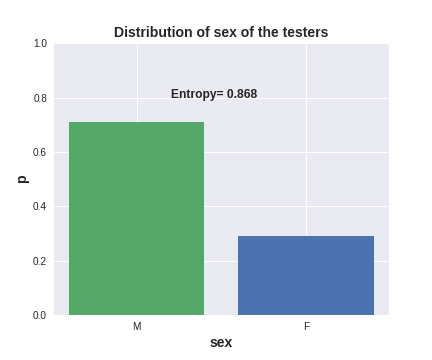
\includegraphics[width=\textwidth]{Bilder/sex_dist.png}
\end{minipage}
\begin{minipage}[t]{0.33\textwidth}
	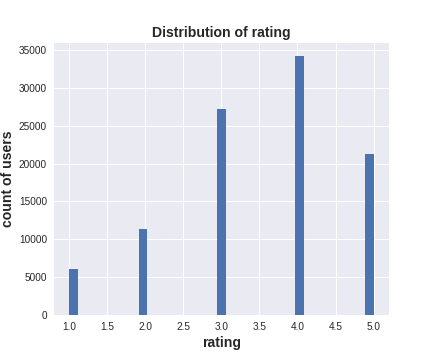
\includegraphics[width=\textwidth]{Bilder/rating_dist.png}
\end{minipage}

\noindent
3.52986
%\begin{figure}[H]
%	\subfigure{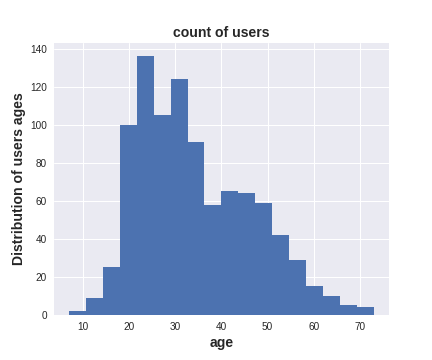
\includegraphics[width=0.49\textwidth]{Bilder/age_dist.png}}
%	\subfigure{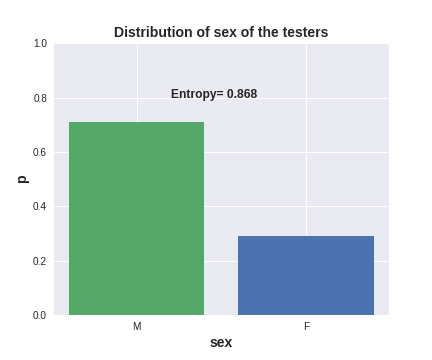
\includegraphics[width=0.49\textwidth]{Bilder/sex_dist.png}}
	%\caption{Titel unterm gesamten Bild}
%\end{figure}
\noindent
It is not a well distributed ages column. I would be better if its better distributed. On the other side the graph shows that there are roughly twice men as woman. This could be crucial for the rating for example more women orientated films. For the rating distribution there is a tendency for bad rated films.\\\\
The target for a regression and a classification task could be the "rating" column.\\\\
For the classification there are multiple classes from (1-5) and the numbers itself for the regression. The input for the training of this model could be the columns to categorize the move. The problem is, that they are no clear correlation between thees columns $|C| = 0.11$ where $C$ is the correlation.
%\section{Potential ethical issues}
%In the user dataset there is the coloum "age" and "occupation". I think that are the only information, which is not ethnical correct. One solution that I could immagen is to divide the coloum "age" into four parts, such as "young", "medium", "adult" and "old".
%There are 21 different names in the coloum "occupation". Divide thees in different other names like "official", "private sector".


\end{document}